\section{Verhalten bei Anregung}
\kopfrechts{Verhalten bei Anregung}%
\subsection{Formelparameter}
In den vorigen Abschnitten wurden die Parameter der Nullklinien des Fitzhugh-Nagumo-Modells folgendermassen definiert:
\(a = -0.7, b = 0.8, \epsilon = 0.8, I_\text{ext} = 0\). Somit werden aus den allgemeinen Nullklinien \[ w = v - \frac{v^3}{3} + I_{ext}\]
und \[w = \frac{v + a}{b}\] die spezifischen Nullklinien \[ w = v - \frac{v^3}{3}\]
und \[w = \frac{v + 0.7}{0.8}.\]
Der stationäre Punkt, welcher von Objekten im Vektorfeld angestrebt werden, befindet sich bei $(1.2 ,-0.6)$.
Der Parameter $I_\text{ext}$ ist als 0 definiert, dies bedeutet, es findet keine Anregung statt.
In Abbildung \ref{fig:Parameter} sind das Vektorfeld und die Nullklinien erkennbar, wenn das Modell nicht angeregt wird.
\begin{figure}
    \centering
    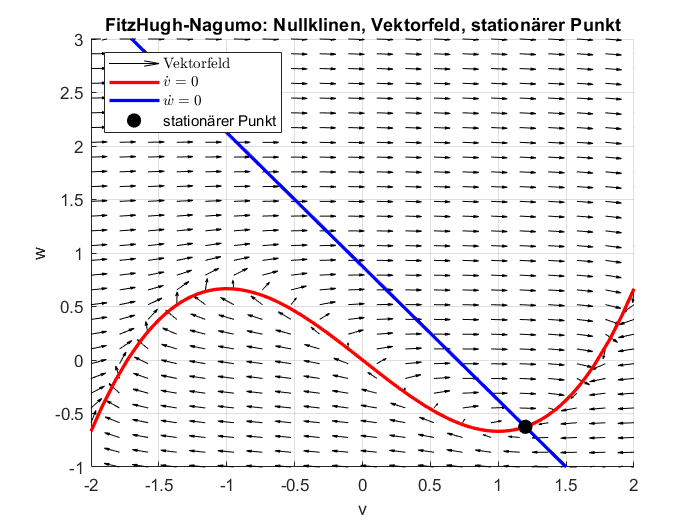
\includegraphics[width=0.9\textwidth]{papers/nerven/Bilder/Anregung1.png}
    \caption{Vektorfeld, Nullklinien und stationärer Punkt ohne Anregung}
    \label{fig:Parameter}
\end{figure}
\subsection{Schwache Anregung}
Wenn das Fitzhugh-Nagumo-Modell angeregt werden soll, muss der Parameter $I_\text{ext}$ verändert werden.
Beispielweise kann $I_\text{ext} = 0.1$ Volt definiert werden.
Dadurch wird die $v$-Nullklinie um 0.1 in positive $w$-Richtung verschoben.
Somit verändern sich die Nullklinien zu \[ w = v - \frac{v^3}{3} + 0.1\]
und \[w = \frac{v + 0.7}{0.8}\] und der stationäre Punkt wandert zu $(1.1 ,-0.5)$.
Der ursprüngliche stationäre Punkt ist jetzt nicht mehr stabil und wird vom Vektorfeld in den neuen stationären Punkt
gezwungen.
Dies geschieht entlang des Vektorfelds, was bei dieser schwachen Anregung nur eine kurze Trajektorie ergibt.
In Abbildung \ref{fig:schwacheAnregung} lässt sich die Trajektorie zwischen den stationären Punkten erkennen, sowie
deren Auslenkung in $v$-Richtung.
Da die Anregung von $I_\text{ext} = 0.1$ sehr schwach ist, fällt auch die Auslenkung der Trajektorie in $v$-Richtung mit 0.2 klein aus und
nimmt sofort wieder ab. 
Dieser Effekt tritt auf, wenn die Nervenzelle mit einer Spannung unterhalb der Schwellenspannung angeregt wird.
\begin{figure}
    \centering
    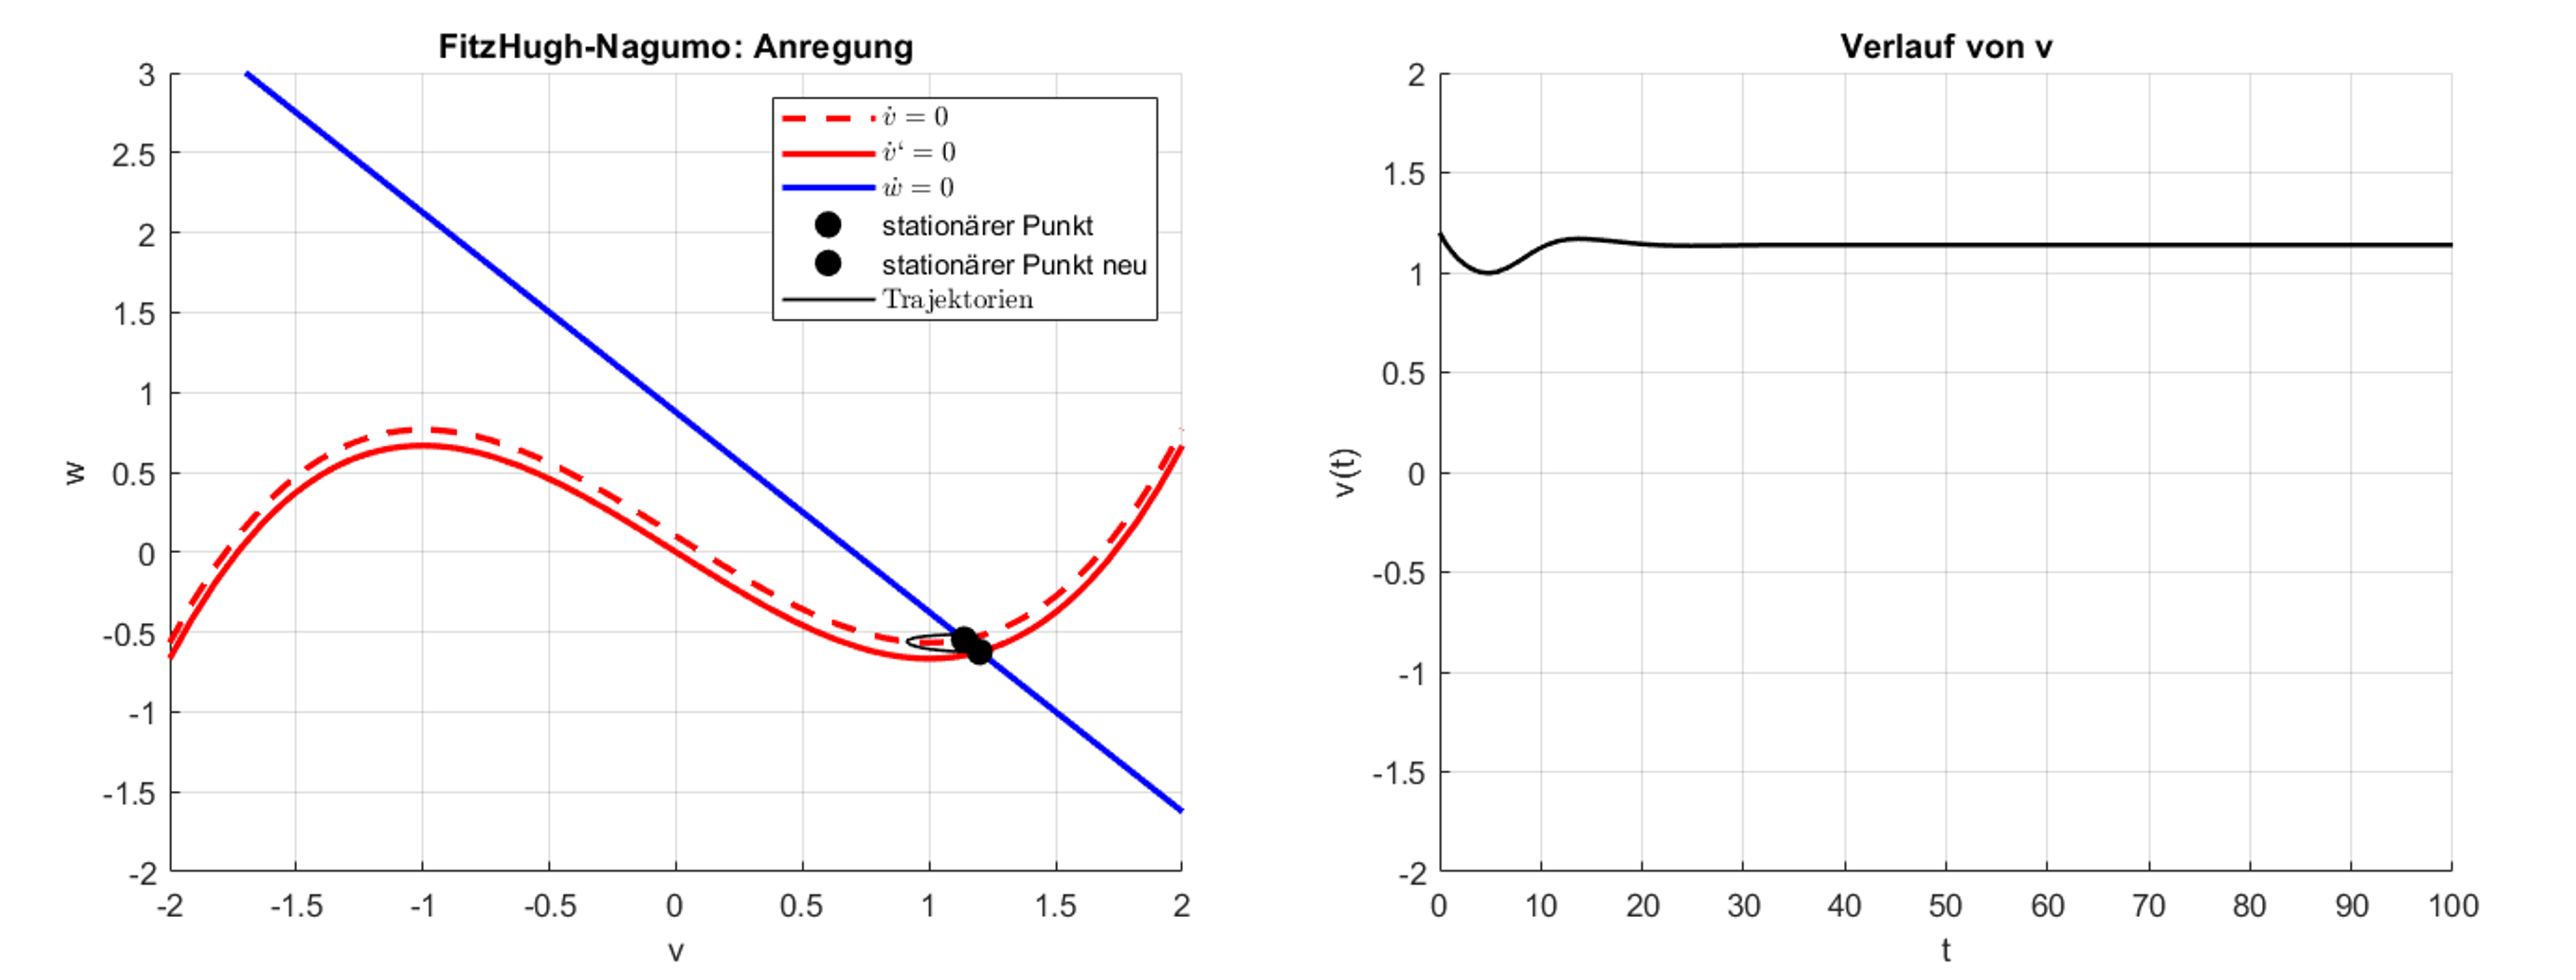
\includegraphics[width=\textwidth]{papers/nerven/Bilder/schwacheAnregung.png}
    \caption{Schwache Anregung des Fitzhugh-Nagumo-Modells}
    \label{fig:schwacheAnregung}
\end{figure}
\subsection{Starke Anregung}
Um den Effekt, der bei einer Nervenzelle bei Anregung über der Schwellenspannung auftritt, beobachten zu können, muss
der Parameter $I_\text{ext}$ erhöht werden.
Beispielweise wird hier $I_\text{ext} = 0.3$ Volt definiert.
Dadurch wird die $v$-Nullklinie um 0.3 in positive $w$-Richtung verschoben.
Somit verändern sich die Nullklinien zu 
\[ w = v - \frac{v^3}{3} + 0.3\]
und \[w = \frac{v + 0.7}{0.8}\] und der stationäre Punkt wandert zu $(1 ,-0.3)$.
Der ursprüngliche stationäre Punkt wird wieder instabil und vom Vektorfeld in den neuen stationären Punkt
gezwungen.
Dies geschieht entlang des Vektorfelds, was bei dieser stärkeren Anregung eine lange Trajektorie ergibt.
In Abbildung \ref{fig:starkeAnregung} lässt sich die Trajektorie zwischen den stationären Punkten erkennen, sowie
deren Auslenkung in $v$-Richtung.
Durch das Vektorfeld muss der ursprüngliche stationäre Punkt, bei einer Anregung von $I_\text{ext} = 0.3$ eine grosse Kurve
beschreiben, um den neuen stationären Punkt zu erreichen.
Die Auslenkung in $v$-Richtung ist dadurch mit $-3$ auch viel grösser und es lässt sich ein impulsartiger Verlauf erkennen.
\begin{figure}
    \centering
    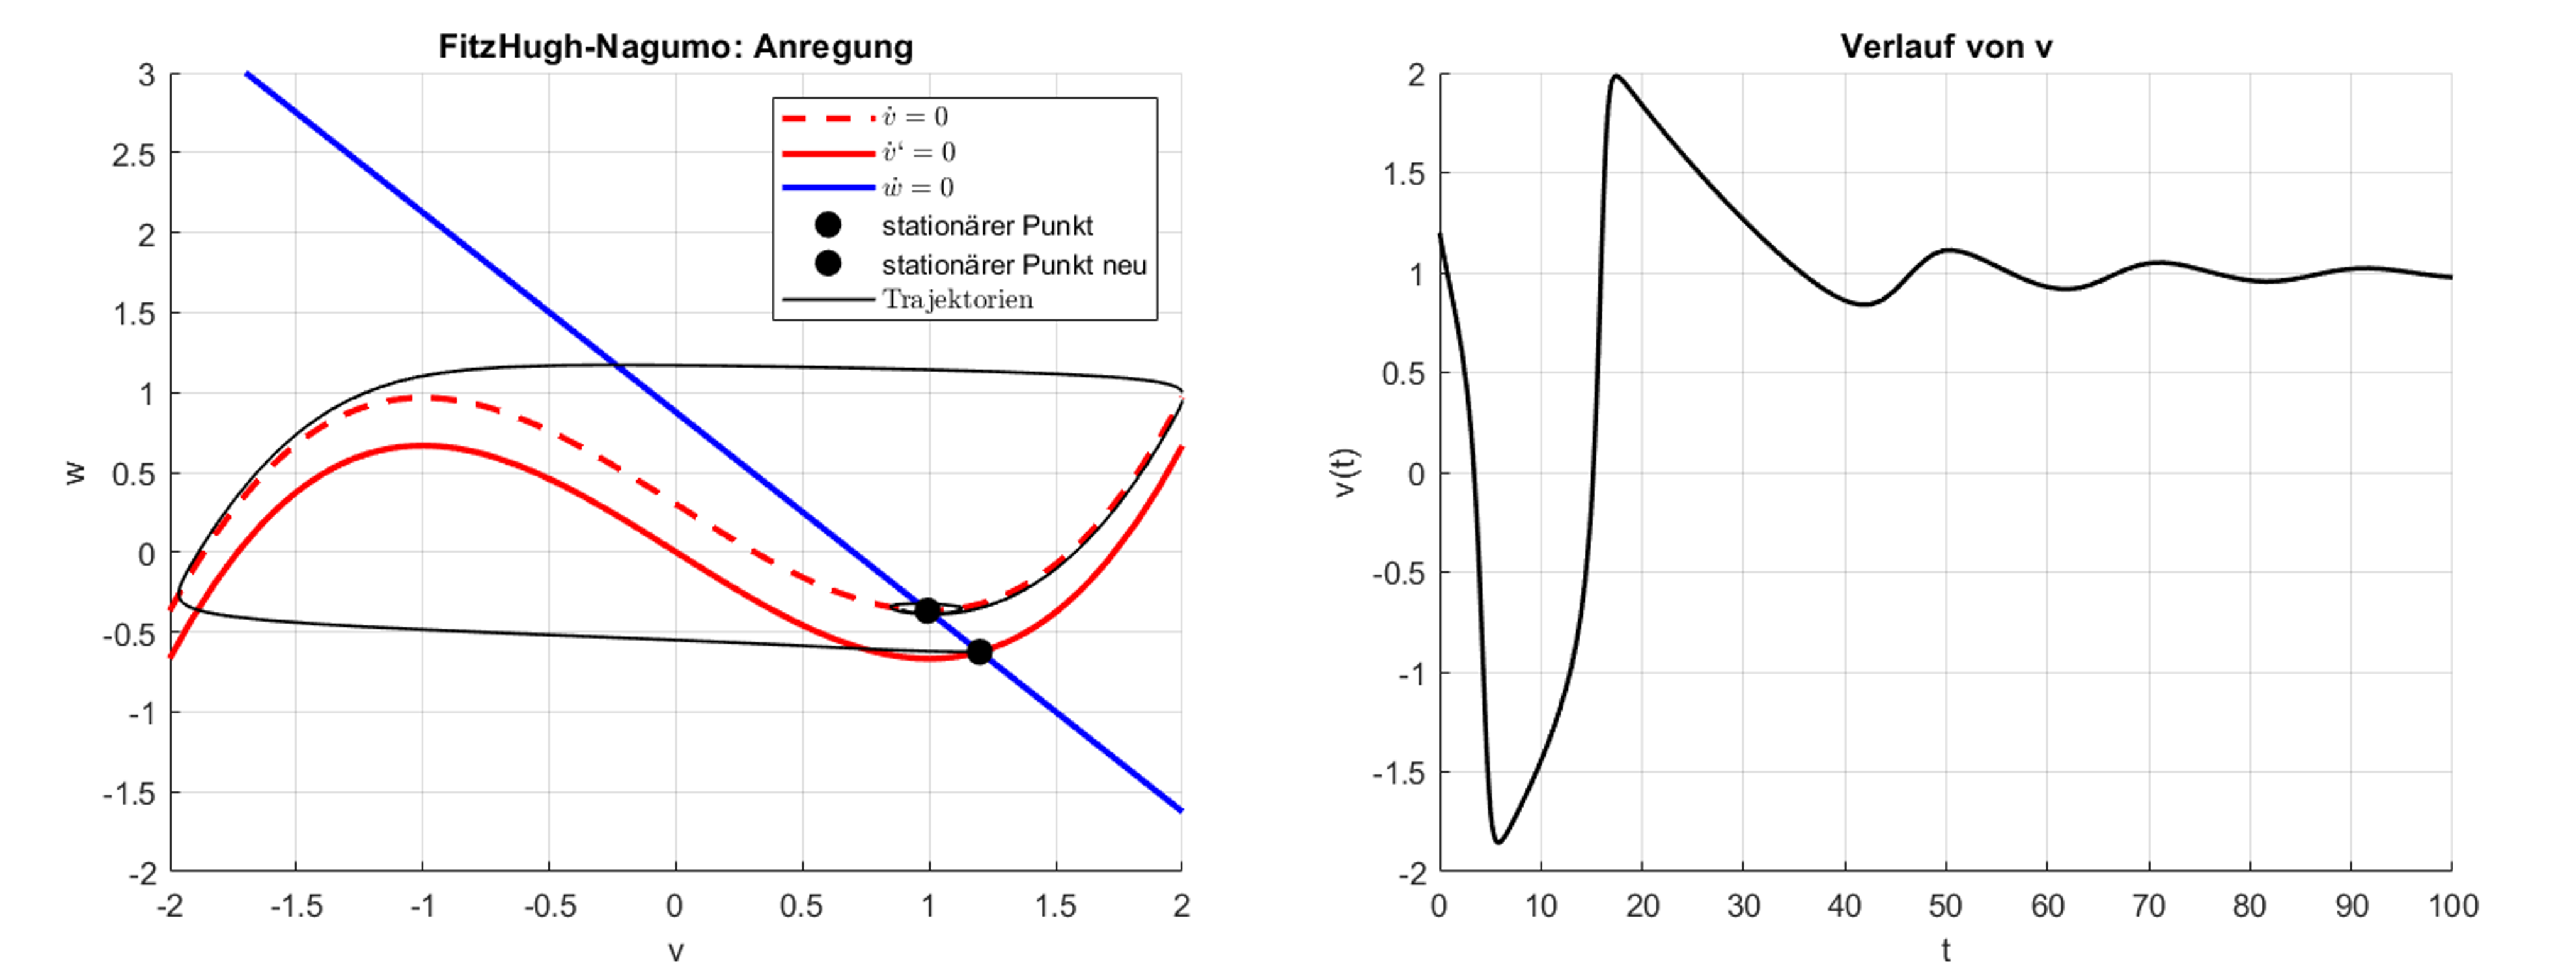
\includegraphics[width=\textwidth]{papers/nerven/Bilder/starkeAnregung.png}
    \caption{Starke Anregung des Fitzhugh-Nagumo-Modells}
    \label{fig:starkeAnregung}
\end{figure}
\subsection{Vergleich mit Aktionspotential}
Der Verlauf der Auslenkung der Trajektorie in $v$-Richtung bei einer starken Anregung des FitzHugh-Nagumo-Modell, lässt
sich mit dem Verlauf des Aktionspotentials der Nervenzelle vergleichen. 
In Abbildung \ref{fig:Vergleich} sind links die Auslenkung in $v$-Richtung und rechts der Verlauf des Aktionspotentials
erkennbar.
Der Verlauf der Auslenkung in $v$-Richtung ist an der $v$-Achse gespiegelt, um die Abbildungen besser vergleichen zu können.
In der Abbildung lassen sich die einzelnen Phasen: Depolarisation, Repolarisation und Hyperpolarisation erkennen, die
sowohl im Verlauf der Auslenkung in $v$-Richtung und im Verlauf des Aktionspotentials auftreten.
Somit kann mit dem Nullklinienmodell des FitzHugh-Nagumo-Modells der Verlauf des Aktionspotentials einer Nervenzelle
dargestellt werden.
\begin{figure}
    \centering
    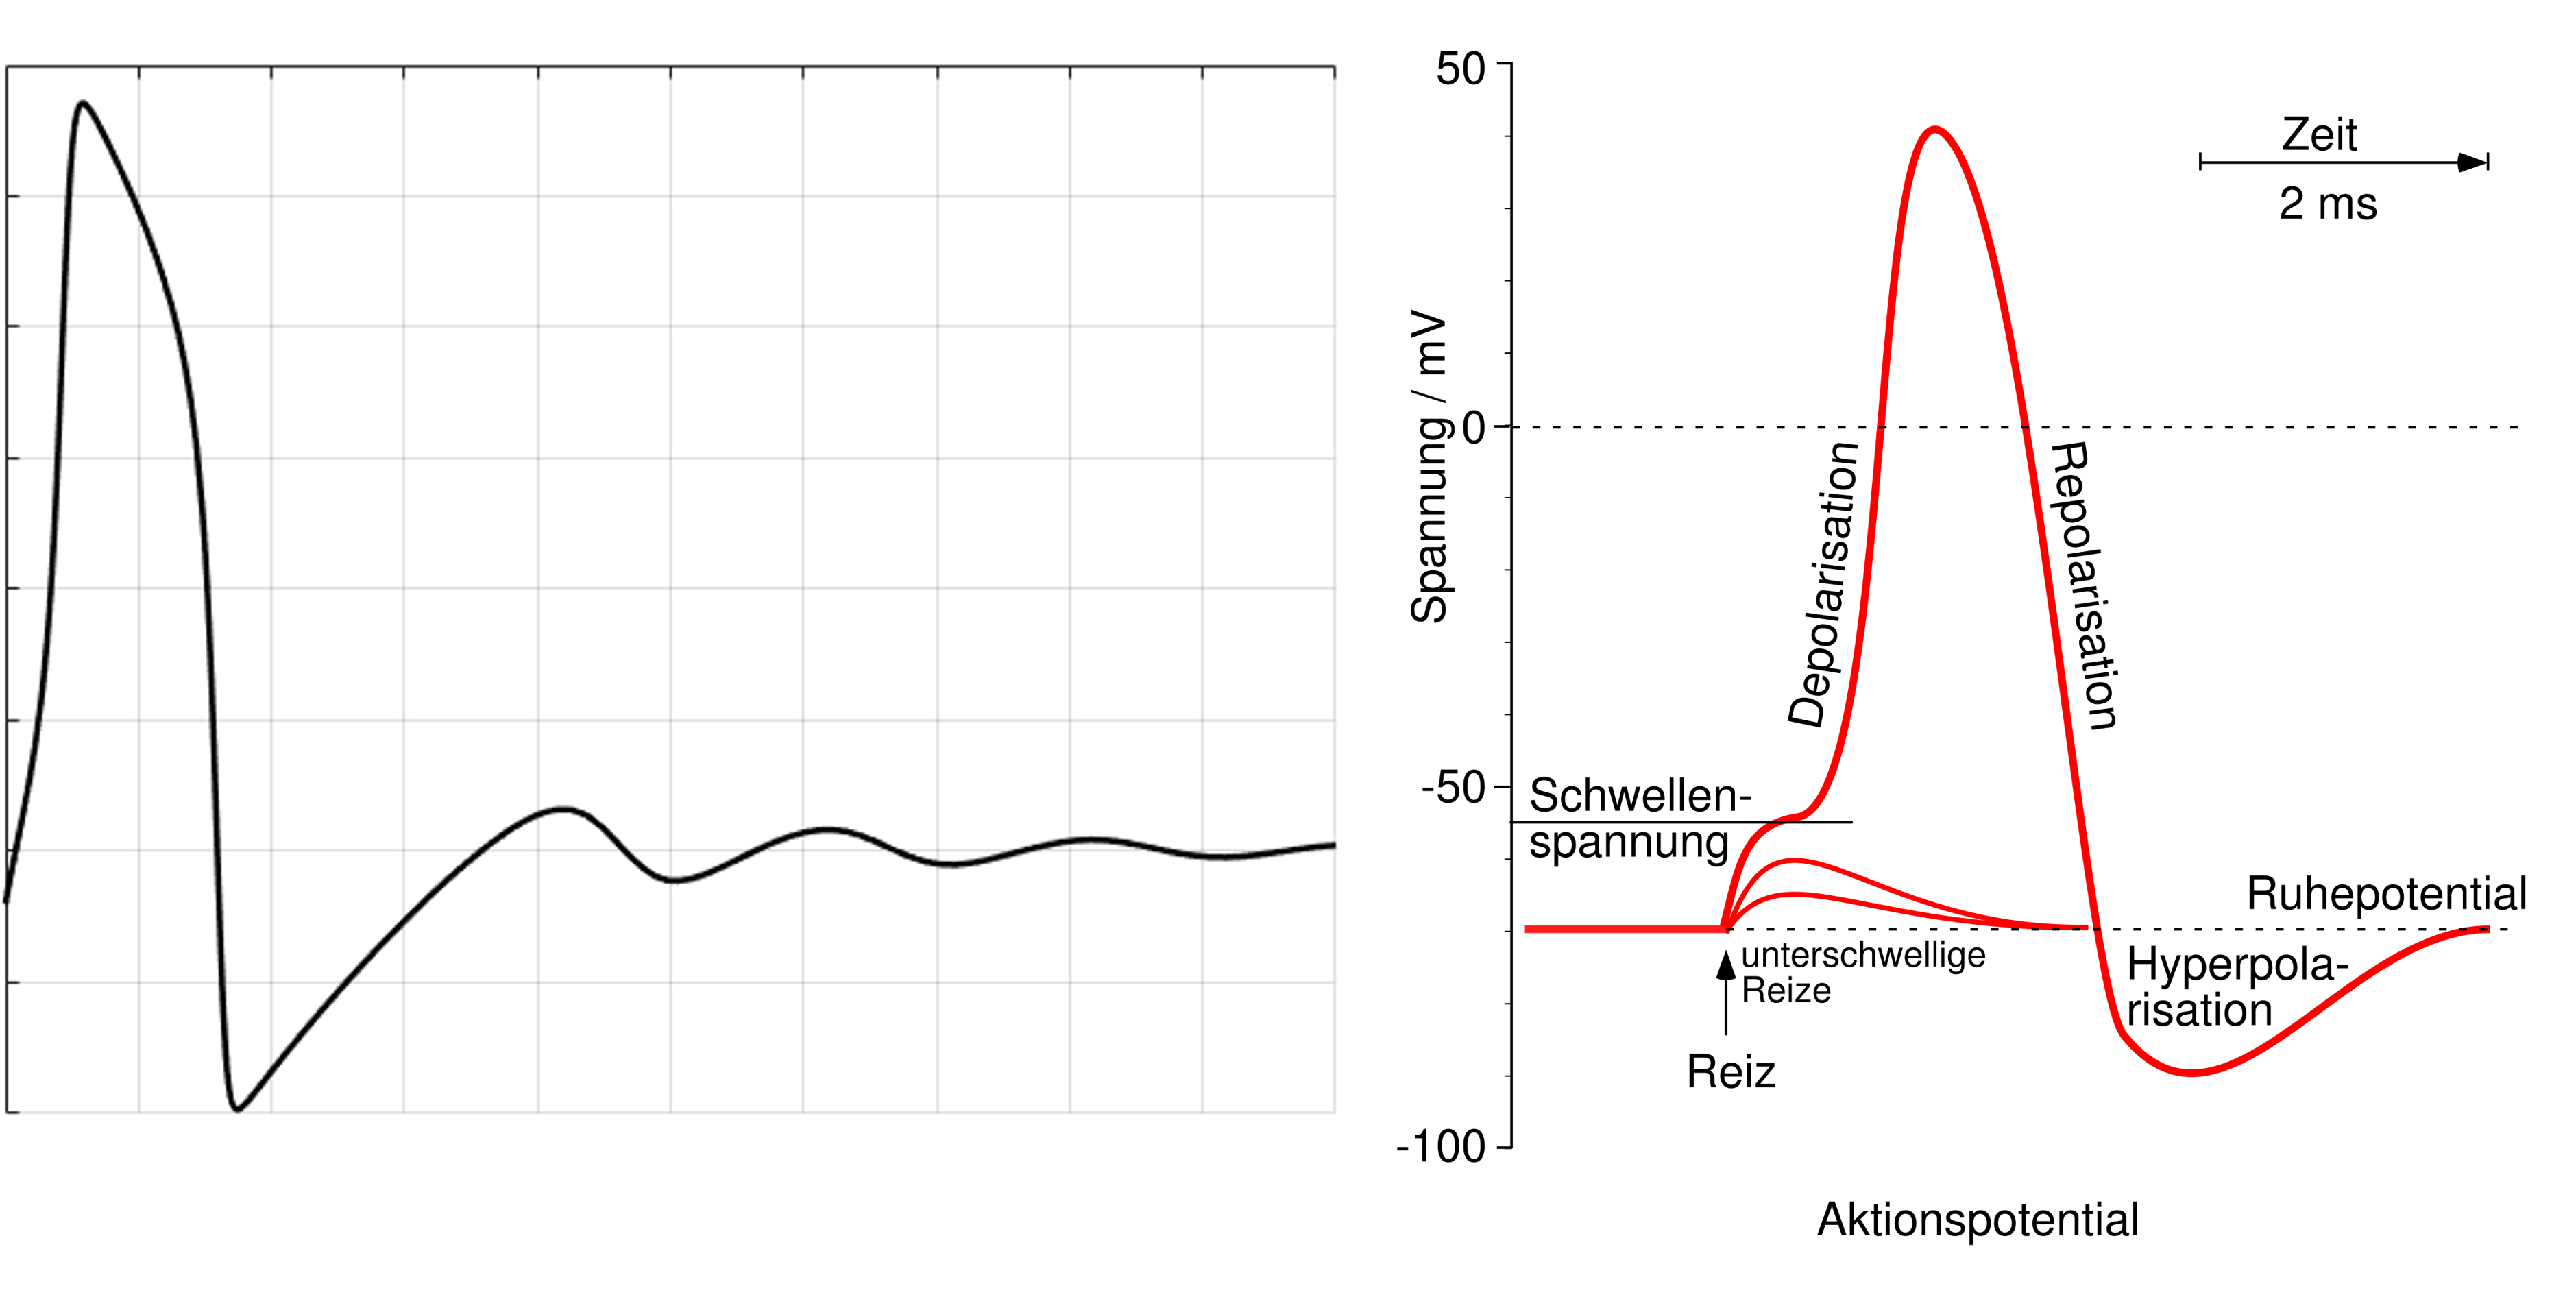
\includegraphics[width=\textwidth]{papers/nerven/Bilder/Vergleich.png}
    \caption{Vergleich $v$-Auslenkung des FitzHugh-Nagumo-Modells mit dem realen Aktionspotential}
    \label{fig:Vergleich}
\end{figure}
